\documentclass[fleqn,11pt]{article}

\usepackage[letterpaper,margin=.75in]{geometry}

\usepackage{amsmath}
\usepackage{booktabs}
\usepackage{graphicx}
\usepackage{listings}
\usepackage{minted}
\usepackage{titling}
\usepackage{xcolor}
\usepackage{tikz}
\usepackage{hyperref}
\usepackage{sectsty}
\usepackage{multicol}
\usepackage{ifthen}
\usepackage{libertine}
\usepackage{inconsolata}

\newcommand{\percent}[1]{\ifthenelse{\equal{#1}{00}}{0}{#1}\%}


\makeatletter
\def\@maketitle{   % custom maketitle 
	{\Large \bfseries \@title}
	\hfill \theauthor
	\smallskip \hrule \bigskip }
    
\hypersetup{
    colorlinks,
    citecolor=black,
    filecolor=black,
    linkcolor=black!70!blue,
    urlcolor=black!40!blue
}

\definecolor{dark-red}{rgb}{.4,0,0}
\definecolor{dark-blue}{rgb}{0,0,.5}
\definecolor{lighter-blue}{rgb}{.4,.4,1}

%\renewcommand{\section}{\@startsection
%   	{section}%                   % the name
%   	{1}%                         % the level
%   	{0mm}%                       % the indent
%   	{.8\baselineskip}%            % the before skip
%   	{0.1\baselineskip}%          % the after skip
%   	{\bfseries}} % the style
\makeatother

\sectionfont{\color{dark-blue}}
\subsectionfont{\color{lighter-blue}}

\setlength{\parindent}{0em}
\setminted{
framesep=2mm,
baselinestretch=1.2,
fontsize=\footnotesize,
%linenos
}

\title{CS 460: Reliable Transport}
\author{Kevin Haroldsen}
\date{}


\begin{document}

\maketitle

\section{Basic Tests}
Each of these tests on the \href{https://github.com/kupiakos/bene}{Bene} simulator was run with a link throughput of 10 Mbps, and a propagation delay of 10 ms.
\subsection{Small File}
The smaller file, \texttt{test.txt}, was transferred with a window size of 3000 bytes.
It's clear, from the data below, that the loss rate has an extremely high effect on the total time needed to transmit the data.
\begin{multicols}{2}
\foreach \x in {00,20,10,50} {
\percent{\x} loss rate:
\inputminted{text}{small-\x-basic.txt}
}
\end{multicols}

\subsection{Large File}
The larger file, \texttt{internet-architecture.pdf}, was transferred with a window size of 10,000 bytes.
Interestingly enough, when exposed to a 50\% loss rate, the effect when compared to the 0\% loss rate is not as drastic as it was for the large file.
This effect is also generally reproducible.
My guess is that with a larger amount of data to work with, and a larger window, an error that occurs in the middle will still likely not largely affect the end.

\clearpage
\begin{multicols}{2}
\foreach \x in {00,50} {
\percent{\x} loss rate:
\inputminted{text}{large-\x-basic.txt}
}
\end{multicols}

\section{Fast Retransmit}
Both of these tests transferred the large file and a 10,000 byte window.
This was easier than expected to implement.
\subsection{With Fast Retransmit}
With fast retransmit, I noticed quite a bit of time was shaved off.
After analyzing individual logs, I noticed that fast retransmit was much more likely to trigger in the beginning or middle of the transmission rather than at the end.
This seemed to mostly be due to the fact that fewer ACK packets will be received when the rest of the file has been transferred, greatly decreasing the chance of many duplicate ACK packets.
\begin{multicols}{2}
\foreach \x in {00,20} {
\percent{\x} loss rate:
\inputminted{text}{large-\x-fast-3.txt}
}
\end{multicols}

\subsection{Without Fast Retransmit}
Obviously, no difference was noticed in the 0\% loss rate scenario.
\begin{multicols}{2}
\foreach \x in {00,20} {
\percent{\x} loss rate:
\inputminted{text}{large-\x-fast-0.txt}
}
\end{multicols}


\section{Experiments}
Using a bandwidth of 10 Mbps, a propagation delay of 10 ms, a queue size of 100, and a loss rate of 0\%, a transfer of the large file was performed with varying window sizes.
The goal was to discover the effect of the TCP window size on throughput and average queuing delay.

As seen below, the window size appears to have a linear effect on the throughput of the connection.
The maximum throughput of the link was 10 Mbps, and as the window size grew closer to that, so the TCP throughput was brought closer to the maximum.
\begin{figure}[h]
\centering
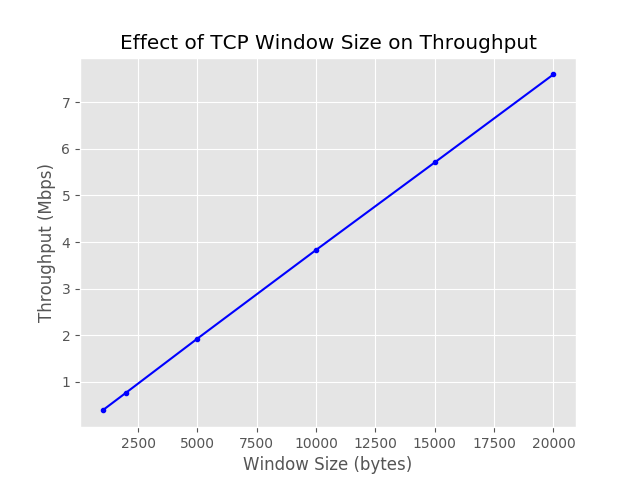
\includegraphics[width=.8\textwidth]{throughput}
\end{figure}

However, the average queuing of packets did not have the same behavior.
As the window size (and throughput) went up, the queuing delay also went up--but more in a quadratic fashion.
In the first window sizes, the queuing delay was next to negligible.
At first, I thought my method of calculating queuing delay was flawed, but then realized it was simply nothing for windows this small.
Even still, it is nearly negligible.
In the end, the highest average queuing delay, for a 20,000-byte window size, was 0.3 milliseconds.

\begin{figure}[h]
\centering
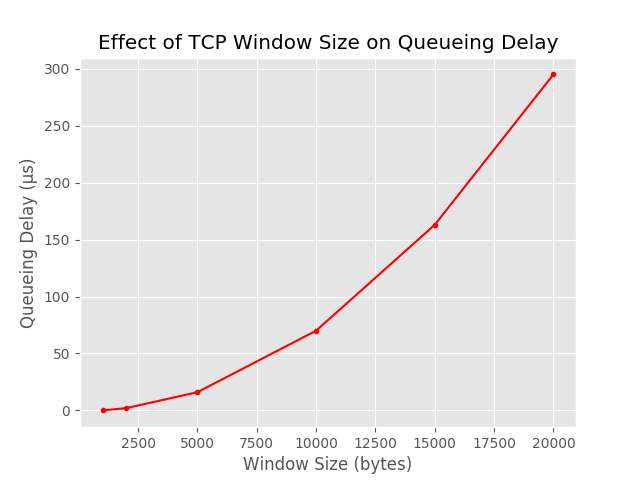
\includegraphics[width=.8\textwidth]{queueing}
\end{figure}

I also ran into another situation that was rather baffling.
It seems that, although the queue size was explicitly defined for this scenario and nothing else, it had no effect on my outcome.
Not once was a link's queue full enough to cause packets to be dropped.

\end{document}
